\documentclass{article}

\usepackage[main,final,nonatbib]{neurips_2026}

\usepackage[utf8]{inputenc}
\usepackage[T1]{fontenc}
\usepackage{hyperref}
\usepackage{url}
\usepackage{booktabs}
\usepackage{amsfonts}
\usepackage{amsmath}
\usepackage{graphicx}
\usepackage{float}
\usepackage{placeins}
\usepackage[font=small,labelfont=bf]{caption}
\usepackage{microtype}
\usepackage{xcolor}

\graphicspath{{../figures/}}
\hypersetup{hidelinks}
\setlength{\textfloatsep}{10pt plus 2pt minus 2pt}
\setlength{\floatsep}{8pt plus 2pt minus 2pt}
\setlength{\intextsep}{8pt plus 2pt minus 2pt}

\title{Scaling GPT Models on TinyStories:\\Training Dynamics, Schedule Sensitivity, and KV-Cache Inference}

\author{%
  Richard Wang \\
  CS290S Deep Learning Practice \\
}

\begin{document}

\maketitle

\begin{abstract}
We study decoder-only GPT language models trained from scratch on TinyStories, spanning 16M to 152M parameters. The implementation uses only PyTorch for the model architecture, causal attention, training loop, generation, and KV-cache path; Hugging Face is restricted to dataset loading, tokenization, and distributed training via Accelerate. Under a fixed 131M-token budget with identical optimizer settings, validation perplexity improves monotonically from 9.68 (16M parameters) to 6.87 (152M parameters) once the learning-rate schedule is appropriate. Controlled diagnostics on the 64M-parameter model reveal that a 5\% warmup ratio reduces its perplexity from 8.23 to 7.64, demonstrating that larger models are more sensitive to schedule configuration under short training horizons. A KV-cache implementation yields a $1.33\times$ generation speedup on the largest model without altering trained parameters.
\end{abstract}

\section{Introduction}

Autoregressive language modeling provides a controlled setting for studying how model capacity, optimization schedule, and inference algorithm interact under fixed compute budgets. We pre-train a family of GPT-style decoders on TinyStories~\cite{eldan2023tinystories}, a synthetic English corpus designed for small-scale language model research, and make three contributions:

\begin{enumerate}
\item A four-model scale comparison (16M--152M parameters) under identical data, optimizer, and token budget, showing that validation perplexity decreases with capacity at the cost of proportionally lower throughput.
\item Controlled single-variable diagnostics explaining why the 64M-parameter model initially underperforms the 34M model: the cause is learning-rate schedule sensitivity rather than insufficient capacity.
\item An inference-time KV-cache modification that achieves $1.33\times$ generation throughput on the largest model without retraining.
\end{enumerate}

All model code, including multi-head causal attention, positional embeddings, and the KV-cache path, is implemented in PyTorch without \texttt{torch.nn.Transformer} or Hugging Face model classes.

\section{Dataset and Preprocessing}

All experiments use the \texttt{roneneldan/TinyStories} dataset accessed through Hugging Face \texttt{datasets}. We cap training at 100{,}000 raw examples and validation at 5{,}000 examples. Tokenization uses the \texttt{roneneldan/TinyStories-33M} BPE tokenizer (vocabulary size 50{,}257). Tokenized examples are concatenated with end-of-sequence separators and packed into contiguous blocks of length 512. Each training item consists of \texttt{input\_ids} and next-token-shifted \texttt{labels}, both of length 512. No additional preprocessing (lowercasing, filtering, or augmentation) is applied.

\begin{table}[!tbp]
\centering
\caption{Dataset statistics. Raw example counts are configured caps; packed blocks are the resulting fixed-length autoregressive training items after concatenation and chunking.}
\label{tab:dataset}
\begin{tabular}{llrrr}
\toprule
Split & Source & Raw examples & Packed blocks & Block length \\
\midrule
Train & TinyStories train & 100{,}000 & 42{,}679 & 512 \\
Validation & TinyStories validation & 5{,}000 & 1{,}943 & 512 \\
\bottomrule
\end{tabular}
\end{table}

The effective training corpus contains $42{,}679 \times 512 = 21.85\text{M}$ tokens per epoch. With 2{,}000 optimizer steps at an effective batch size of 128 sequences, each run processes $131.07\text{M}$ tokens total, corresponding to approximately 6 passes over the packed training set.

\section{Model Architecture}

The model is a decoder-only Transformer implemented in \texttt{gpt.py}. Each variant consists of: (1)~token embeddings and learned absolute positional embeddings, (2)~$L$ pre-norm Transformer blocks with causal multi-head self-attention and GELU-activated feed-forward networks of width $4d_{\mathrm{model}}$, (3)~residual connections around each sub-layer, (4)~a final layer normalization, and (5)~a language-modeling head with weights tied to the token embedding matrix. Dropout of 0.1 is applied to attention weights and residual paths in all variants.

\begin{table}[!tbp]
\centering
\caption{Model configurations. All variants share context length 512, vocabulary 50{,}257, tied embeddings, and dropout 0.1. Parameter counts include the shared embedding matrix.}
\label{tab:architecture}
\begin{tabular}{lrrrrr}
\toprule
Model & Layers & Heads & $d_{\mathrm{model}}$ & Head dim & Parameters \\
\midrule
Tiny & 4 & 4 & 256 & 64 & 16.16M \\
Small & 8 & 6 & 384 & 64 & 33.69M \\
Medium & 12 & 8 & 512 & 64 & 63.82M \\
Large & 16 & 12 & 768 & 64 & 152.40M \\
\bottomrule
\end{tabular}
\end{table}

For the KV-cache experiment (Section~\ref{sec:kv-cache}), the attention module is extended to accept and return cached key--value tensors of shape $[B, H, T_{\mathrm{cached}}, d_h]$. During cached generation, the full prompt is processed in a single forward pass to populate the cache; each subsequent token computes queries only for the new position and attends over the concatenation of cached and current keys/values. The training path is unmodified: cache use is rejected when labels are supplied, ensuring that the comparison isolates inference-time computation reuse.

\clearpage
\section{Training Setup}

Training uses Hugging Face Accelerate with 4 NVIDIA TITAN RTX GPUs and NCCL collective communication. Each TITAN RTX is a Turing GPU with 24 GB GDDR6 memory, 4{,}608 CUDA cores, 576 Tensor Cores, and 672 GB/s memory bandwidth \cite{nvidiatitanrtx}. All four model sizes share identical optimizer, scheduler, batch configuration, and token budget. The effective batch size is $4 \times 8 \times 4 \times 512 = 65{,}536$ tokens per optimizer step (4 devices, per-device batch 8, gradient accumulation 4, sequence length 512). Each run executes 2{,}000 steps, consuming $131.07\text{M}$ tokens.

\begin{table}[H]
\centering
\small
\caption{Training hyperparameters for the primary scale comparison. All four model sizes use these settings identically.}
\label{tab:training}
\begin{tabular}{ll}
\toprule
Hyperparameter & Value \\
\midrule
Optimizer & AdamW ($\beta_1{=}0.9$, $\beta_2{=}0.95$) \\
Peak learning rate & $8 \times 10^{-4}$ \\
Weight decay & 0.1 \\
LR schedule & Cosine decay \\
Warmup ratio & 0.02 (40 steps) \\
Max training steps & 2{,}000 \\
Effective batch size & 128 sequences (65{,}536 tokens) \\
Precision & fp16 mixed precision \\
Gradient clipping & 1.0 (global $\ell_2$ norm) \\
Evaluation interval & every 200 steps \\
Max evaluation batches & 100 \\
Hardware & 4$\times$ NVIDIA TITAN RTX, NCCL backend \\
\bottomrule
\end{tabular}
\end{table}

Generation during validation uses temperature 0.9, top-$k$ 50, and nucleus sampling with $p{=}0.95$. Checkpoints are saved every 1{,}000 steps and at training completion.
\FloatBarrier

\section{Results}

\subsection{Scale Comparison}

Figure~\ref{fig:loss-curves} shows training and validation loss for the four model sizes. Two patterns emerge. First, larger models start with higher validation loss due to slower initial convergence relative to their capacity. Second, the Large model crosses below all smaller models after approximately 1{,}000 steps and achieves the lowest final loss. Figure~\ref{fig:ppl-curves} shows the corresponding perplexity trajectories.

\begin{figure}[H]
\centering
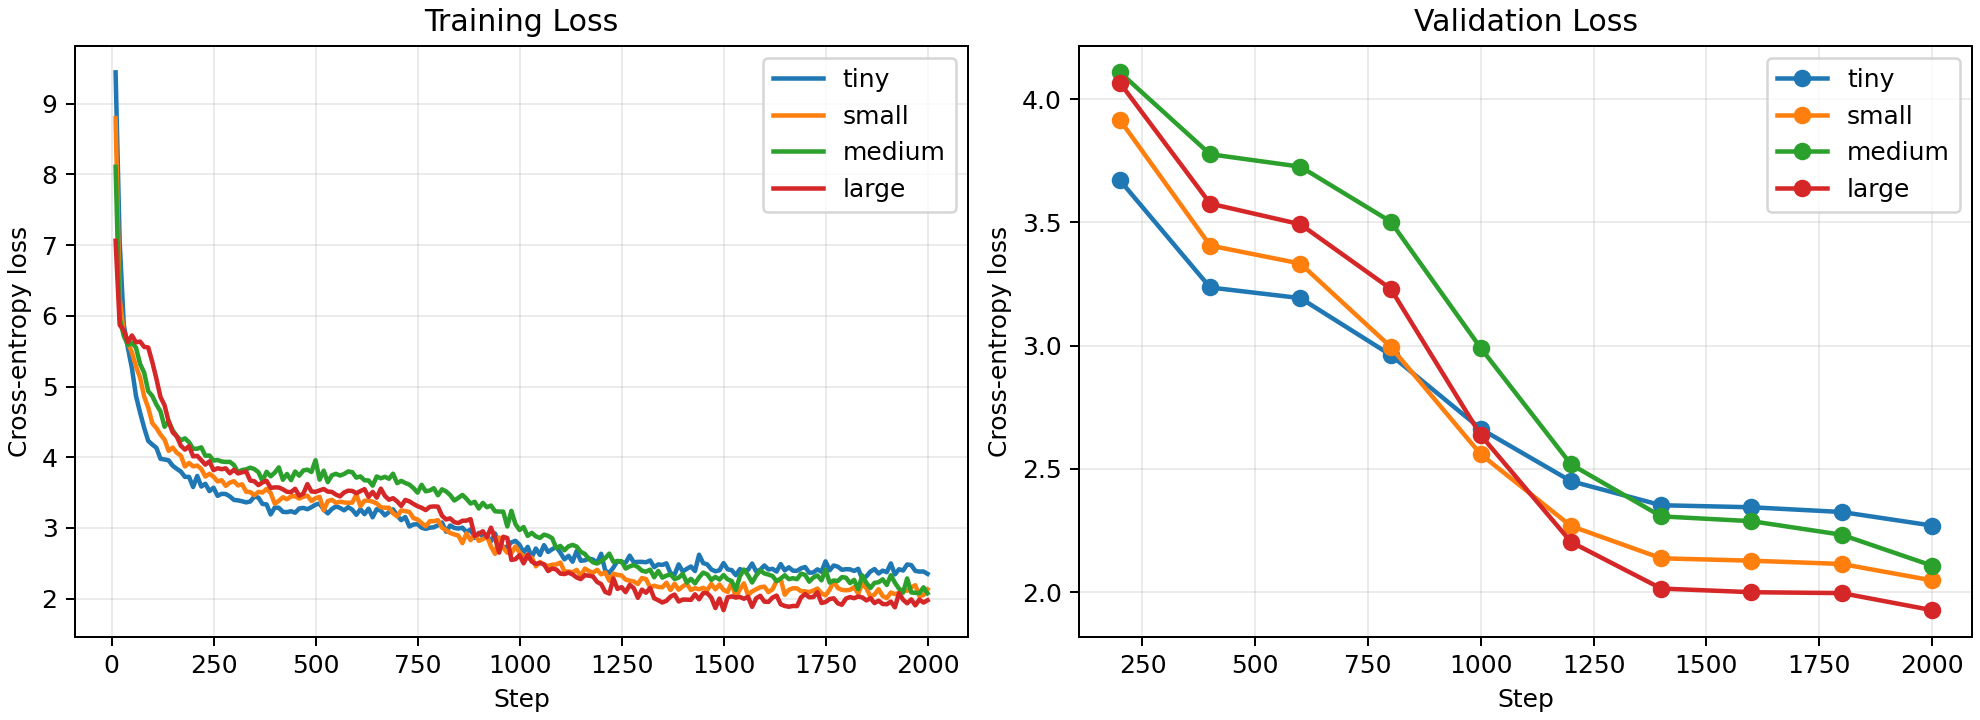
\includegraphics[width=\linewidth]{basic_loss_curves.png}
\caption{Training and validation loss across model sizes. All runs use identical data, optimizer, and 131M-token budget. The Large model converges to the lowest validation loss despite starting highest. The Medium baseline (untuned schedule) finishes above Small.}
\label{fig:loss-curves}
\end{figure}

\begin{figure}[H]
\centering
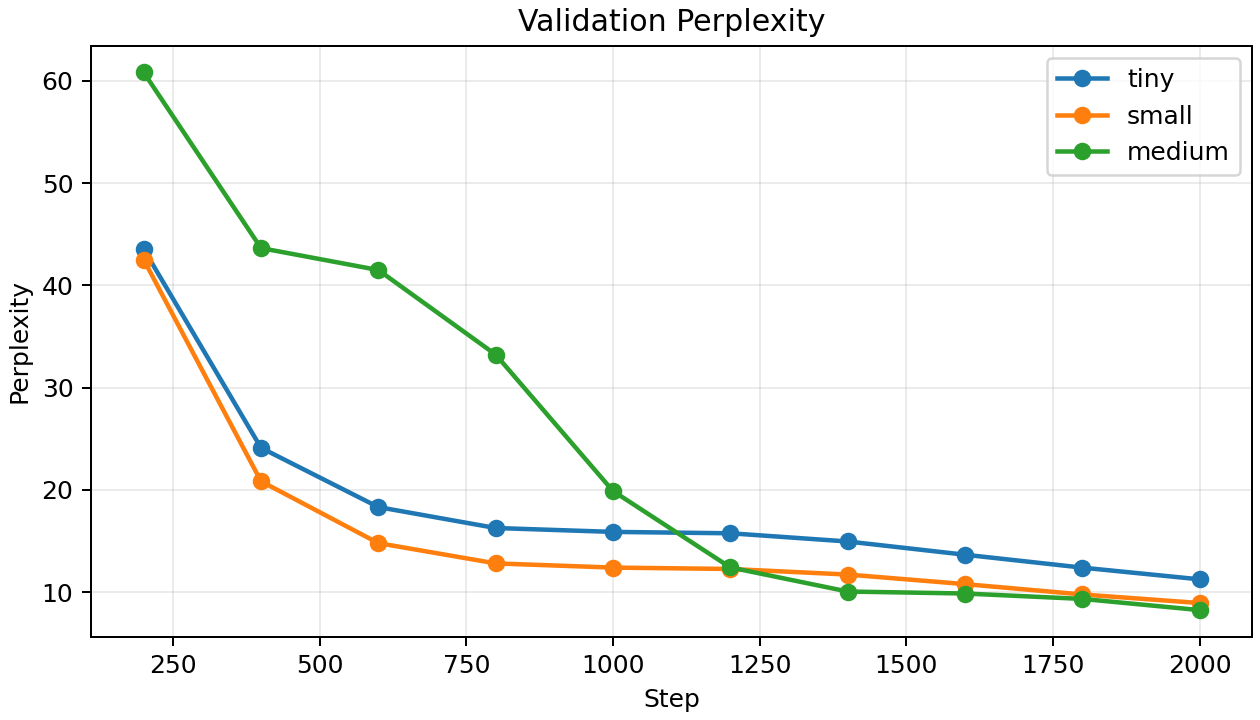
\includegraphics[width=0.70\linewidth]{basic_perplexity_curves.png}
\caption{Validation perplexity over training. Perplexity decreases monotonically with model size except for the untuned Medium run, which finishes above Small due to schedule sensitivity (Section~\ref{sec:diagnostics}).}
\label{fig:ppl-curves}
\end{figure}

\begin{table}[H]
\centering
\small
\caption{Final metrics for the primary scale comparison (2{,}000 steps, 131.07M tokens). Throughput is measured end-to-end including evaluation. Peak memory is \texttt{torch.cuda.max\_memory\_allocated} per device.}
\label{tab:main-results}
\begin{tabular}{lrrrrrr}
\toprule
Model & Params & Runtime & Tokens/s & Peak mem. & Val loss & Val PPL \\
\midrule
Tiny & 16.16M & \textbf{7.97 min} & \textbf{274{,}182} & \textbf{3.79 GiB} & 2.270 & 9.68 \\
Small & 33.69M & 15.20 min & 143{,}745 & 4.92 GiB & 2.048 & 7.75 \\
Medium & 63.82M & 26.65 min & 81{,}969 & 6.64 GiB & 2.108 & 8.23 \\
Large & 152.40M & 51.81 min & 42{,}164 & 10.68 GiB & \textbf{1.927} & \textbf{6.87} \\
\bottomrule
\end{tabular}
\end{table}

Table~\ref{tab:main-results} quantifies the scaling trade-off. Moving from Tiny to Large reduces validation perplexity by 29\% (9.68$\to$6.87) while reducing throughput by 6.5$\times$ and increasing peak memory by 2.8$\times$. The anomalous Medium result---worse perplexity than Small despite 1.9$\times$ more parameters and lower training loss---motivates the diagnostic study below.
\FloatBarrier

\subsection{Medium-Model Diagnostics}
\label{sec:diagnostics}

The Medium baseline achieves lower final training loss (2.075) than Small (2.132) but higher validation loss (2.108 vs.\ 2.048), indicating an optimization-generalization mismatch rather than insufficient capacity. We run four controlled diagnostics, each changing a single hyperparameter while holding the model, data, seed, GPU count, and token budget fixed.

\begin{figure}[H]
\centering
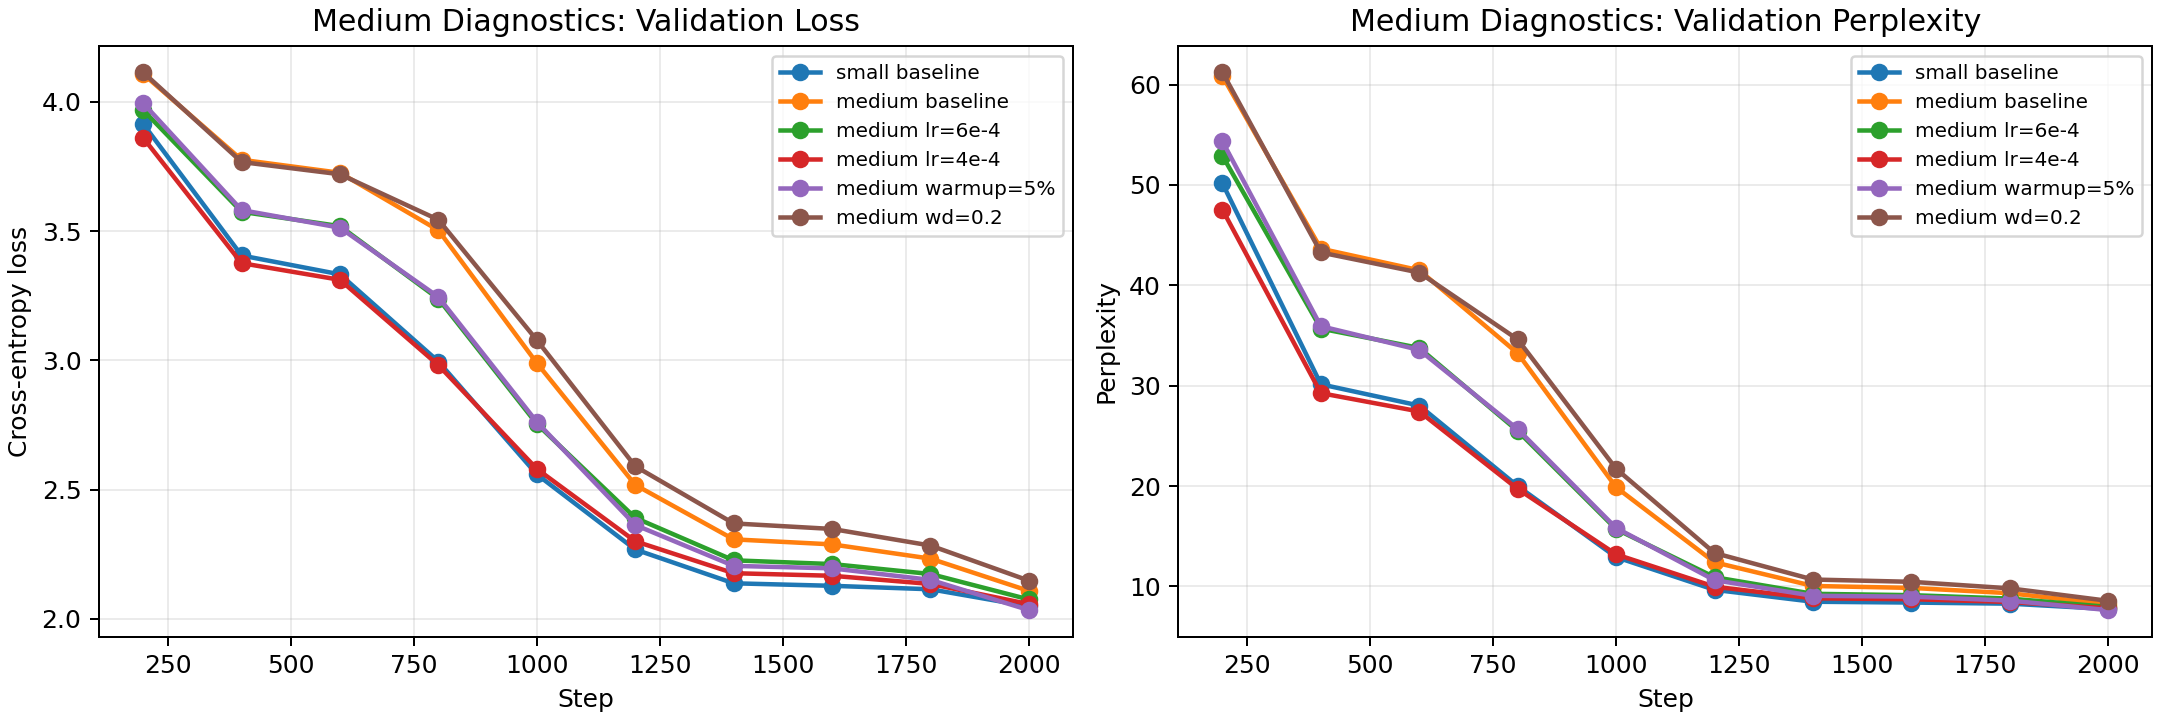
\includegraphics[width=\linewidth]{medium_diagnostic_curves.png}
\caption{Validation loss curves for Medium diagnostics. Reducing the learning rate or extending warmup improves generalization; increasing weight decay degrades it.}
\label{fig:medium-diagnostic}
\end{figure}

\begin{table}[H]
\centering
\small
\caption{Controlled Medium diagnostics. Each run modifies one hyperparameter from the Medium baseline. The Small baseline is included for reference.}
\label{tab:medium-diagnostic}
\begin{tabular}{llrr}
\toprule
Configuration & Modification & Val loss & Val PPL \\
\midrule
Small baseline & 33.69M params, same schedule & 2.048 & 7.75 \\
Medium baseline & LR $8{\times}10^{-4}$, warmup 2\%, wd 0.1 & 2.108 & 8.23 \\
Medium LR $6{\times}10^{-4}$ & Lower peak LR & 2.075 & 7.96 \\
Medium LR $4{\times}10^{-4}$ & Lower peak LR & 2.057 & 7.82 \\
Medium warmup 5\% & Warmup 40$\to$100 steps & 2.033 & 7.64 \\
Medium wd 0.2 & Stronger weight decay & 2.147 & 8.56 \\
\bottomrule
\end{tabular}
\end{table}

The results (Table~\ref{tab:medium-diagnostic}) support a clear interpretation: the Medium model's underperformance is schedule-driven. Halving the learning rate from $8{\times}10^{-4}$ to $4{\times}10^{-4}$ improves perplexity from 8.23 to 7.82. Extending warmup from 2\% to 5\% yields the best result (7.64), surpassing the Small baseline. Conversely, increasing weight decay to 0.2 worsens perplexity to 8.56, ruling out under-regularization as the cause. The mechanism is consistent with known sensitivity of larger models to learning-rate warmup under short training horizons~\cite{radford2018gpt}: with only 40 warmup steps, the 64M-parameter model receives large gradient updates before its loss landscape has stabilized.

These are single-seed results and should be interpreted as measured trends rather than statistically robust claims.
\FloatBarrier

\subsection{Generated Samples}

Table~\ref{tab:samples} summarizes generation quality across the scale ladder. All samples use the prompt \emph{``Once upon a time''} with temperature 0.9, top-$k$ 50, and $p{=}0.95$.

\begin{table}[H]
\centering
\scriptsize
\caption{Representative generated samples and qualitative assessment. Each model produces three 512-token continuations from the same prompt; examples are condensed from archived full-text outputs.}
\label{tab:samples}
\begin{tabular}{lp{0.40\linewidth}p{0.40\linewidth}}
\toprule
Model & Representative archived examples & Generation characteristics \\
\midrule
Tiny & A family trip reaches an airport but the action drifts; Sue finds a melting snowman; Lily finds a tree with an axe. & Maintains child-story register, but destination, object references, and causal links are often confused. \\
Small & Lily visits a park with swings, slides, and a butterfly; Lily finds a magic chain; Lily finds a shiny garden gem. & More locally coherent event sequences and clearer nouns/actions than Tiny, though object roles can remain under-specified. \\
Medium & Lily sees a butterfly and cricket; Timmy breaks a toy car; Lily plays near a swing until rain starts. & Fluent TinyStories-style prose with better event progression, but still contains semantic oddities and imperfect causality. \\
Large & Lily receives a box of powder; Lily shares a red ball with Sam; Lily finds leaves that turn into fire. & Best sample achieves a complete sharing-story arc; other samples are fluent but still show repetition or semantic inconsistency. \\
\bottomrule
\end{tabular}
\end{table}

Qualitatively, generation coherence improves with model size: Tiny produces grammatical but causally disconnected text, while Large occasionally produces complete story arcs. All models exhibit repetition at 512 tokens, consistent with the limited training budget and absence of repetition penalties.
\FloatBarrier

\subsection{KV-Cache Inference Benchmark}
\label{sec:kv-cache}

We evaluate the KV-cache implementation on the Large model checkpoint (step 2{,}000). The benchmark uses three prompts of varying length, generates 512 new tokens per prompt, and measures wall-clock time over 5 iterations after 3 warmup iterations on a single GPU. Both modes use identical sampling parameters (temperature 0.9, top-$k$ 50, $p{=}0.95$) and the same random seed, producing bitwise-identical outputs.

\begin{table}[H]
\centering
\small
\caption{Single-GPU generation benchmark on the Large model (152.40M parameters). Each mode generates 7{,}680 tokens total (3 prompts $\times$ 512 tokens $\times$ 5 iterations).}
\label{tab:kv-cache}
\begin{tabular}{lrrrrr}
\toprule
Mode & Tokens & Wall time & ms/token & Tokens/s & Peak mem. \\
\midrule
No cache & 7{,}680 & 102.59\,s & 13.36 & 74.86 & 0.774 GiB \\
KV cache & 7{,}680 & \textbf{77.24\,s} & \textbf{10.06} & \textbf{99.43} & \textbf{0.690 GiB} \\
\midrule
\multicolumn{2}{l}{Speedup} & \textbf{$1.33\times$} & & & \\
\bottomrule
\end{tabular}
\end{table}

The KV cache reduces generation time by 24.7\% (Table~\ref{tab:kv-cache}). The speedup arises because the no-cache path recomputes all key--value projections for the full prefix at every decoding step, yielding $O(T^2 \cdot d)$ total attention computation for $T$ generated tokens. The cached path computes projections only for the new token and concatenates with stored tensors, reducing per-step attention to $O(T \cdot d)$. Peak memory is slightly lower for the cached path in this configuration because the no-cache path materializes the full $T \times T$ attention matrix at the final step, while the cached path processes only a $1 \times T$ attention vector.

The benchmark is limited to one model size, one GPU, one generation length, and batch size 1. The measured $1.33\times$ speedup is specific to these conditions; longer sequences would yield larger speedups as the quadratic cost of recomputation grows.
\FloatBarrier

\section{Analysis and Discussion}

\paragraph{Scaling behavior.} The results confirm that model capacity improves validation perplexity on TinyStories under a fixed 131M-token budget, with diminishing throughput. The Tiny-to-Small transition yields the largest perplexity-per-parameter improvement (1.93 PPL reduction for 17.5M additional parameters), while Small-to-Large yields 0.88 PPL reduction for 118.7M parameters. This sub-linear scaling is expected given the limited dataset diversity and short training horizon.

\paragraph{Schedule sensitivity.} The Medium anomaly demonstrates that scaling laws assume appropriate optimization. The Medium model's 12 layers and 512-dimensional representations create a deeper loss landscape that requires more conservative initial updates. With only 40 warmup steps (2\% of 2{,}000), the optimizer applies near-peak learning rate before the model has reached a stable training regime. Extending warmup to 100 steps (5\%) resolves the issue entirely, reducing Medium perplexity below the Small baseline. This finding is practically relevant: practitioners scaling model size under fixed step budgets should co-scale warmup duration.

\paragraph{KV-cache mechanism.} Standard autoregressive generation without caching performs redundant computation: at step $t$, it recomputes key--value projections for positions $1$ through $t{-}1$ that were already computed at step $t{-}1$. The KV cache eliminates this redundancy by storing and reusing these projections. The $1.33\times$ measured speedup for 512-token generation on a 16-layer model is consistent with the expected benefit: the cache eliminates $O(T)$ redundant projection operations per step, with the constant factor depending on the ratio of attention computation to other forward-pass costs (embeddings, FFN, layer norms).

\paragraph{Limitations.} All training runs use a single seed; reported differences are point estimates without confidence intervals. The TinyStories subset is small and low-diversity relative to standard pre-training corpora, limiting generalization of scaling conclusions. The KV-cache benchmark uses batch size 1 and a single generation length; memory--throughput trade-offs at larger batch sizes are not characterized.

\section{Conclusion}

We implement GPT pre-training from scratch and evaluate model scaling and KV-cache inference on TinyStories. Three findings emerge: (1)~validation perplexity improves from 9.68 to 6.87 across a 16M--152M parameter ladder under fixed compute; (2)~the 64M-parameter model's initial underperformance is fully explained by learning-rate schedule sensitivity, with 5\% warmup reducing its perplexity to 7.64; (3)~KV caching yields $1.33\times$ generation speedup by eliminating redundant key--value recomputation. The results demonstrate that scaling benefits require co-adaptation of the optimization schedule, and that inference-time algorithmic improvements are orthogonal to model quality.

\begin{thebibliography}{9}

\bibitem{radford2018gpt}
Alec Radford, Karthik Narasimhan, Tim Salimans, and Ilya Sutskever.
\newblock Improving language understanding by generative pre-training.
\newblock Technical report, OpenAI, 2018.

\bibitem{eldan2023tinystories}
Ronen Eldan and Yuanzhi Li.
\newblock TinyStories: How small can language models be and still speak coherent English?
\newblock \emph{arXiv preprint arXiv:2305.07759}, 2023.

\bibitem{huggingfaceaccelerate}
Hugging Face.
\newblock Accelerate documentation.
\newblock \url{https://huggingface.co/docs/accelerate}.

\bibitem{nvidiatitanrtx}
NVIDIA.
\newblock NVIDIA TITAN RTX specifications.
\newblock \url{https://www.nvidia.com/en-us/titan/titan-rtx/}.

\end{thebibliography}

\end{document}
